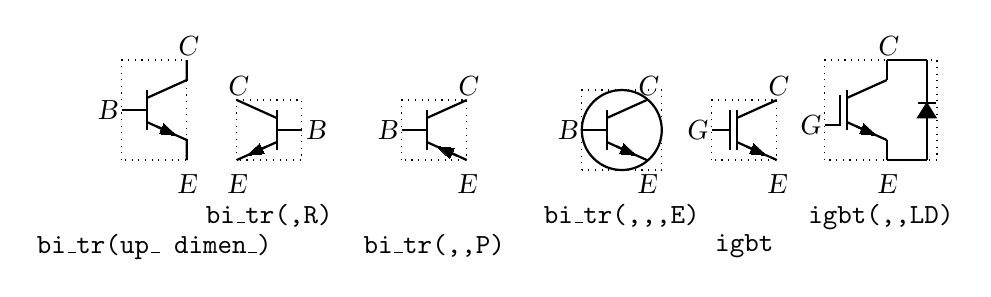
\begin{tikzpicture}[scale=2.54]
% dpic version 2020.03.01 option -g for TikZ and PGF 1.01
\ifx\dpiclw\undefined\newdimen\dpiclw\fi
\global\def\dpicdraw{\draw[line width=\dpiclw]}
\global\def\dpicstop{;}
\dpiclw=0.8bp
\dpiclw=0.8bp
\dpicdraw (0.1625,0)
 --(0.1625,0.1)
 --(0.158796,0.101667)\dpicstop
\dpicdraw (0.1625,0.5)
 --(0.1625,0.4)
 --(0.158796,0.398333)\dpicstop
\dpicdraw (-0.0375,0.15)
 --(-0.0375,0.35)\dpicstop
\dpicdraw (-0.1625,0.25)
 --(-0.0375,0.25)\dpicstop
\dpicdraw (0.1625,0.1)
 --(-0.0375,0.19)\dpicstop
\filldraw[line width=0bp](0.025108,0.131366)
 --(0.1125,0.1225)
 --(0.047906,0.182028) --cycle\dpicstop
\dpicdraw (0.096479,0.129709)
 --(0.0125,0.1675)\dpicstop
\dpicdraw (0.1625,0.4)
 --(-0.0375,0.31)\dpicstop
\dpiclw=0.4bp
\dpicdraw[dotted](-0.1625,0) rectangle (0.1625,0.5)\dpicstop
\dpiclw=0.8bp
\draw (0.1625,-0.05) node[below=-2bp]{\hbox{\sl E}};
\draw (-0.1625,0.25) node[left=-2bp]{\hbox{\sl B}};
\draw (0.1625,0.5) node[above=-2bp]{\hbox{\sl C}};
\draw (0,-0.35) node[below=-2bp]{{\tt bi\_tr(up\_ dimen\_)}};
\dpicdraw (0.6125,0.05)
 --(0.6125,0.25)\dpicstop
\dpicdraw (0.7375,0.15)
 --(0.6125,0.15)\dpicstop
\dpicdraw (0.4125,0)
 --(0.6125,0.09)\dpicstop
\filldraw[line width=0bp](0.527094,0.082028)
 --(0.4625,0.0225)
 --(0.549892,0.031366) --cycle\dpicstop
\dpicdraw (0.478521,0.029709)
 --(0.5625,0.0675)\dpicstop
\dpicdraw (0.4125,0.3)
 --(0.6125,0.21)\dpicstop
\dpiclw=0.4bp
\dpicdraw[dotted](0.4125,0) rectangle (0.7375,0.3)\dpicstop
\dpiclw=0.8bp
\draw (0.4125,-0.05) node[below=-2bp]{\hbox{\sl E}};
\draw (0.7375,0.15) node[right=-2bp]{\hbox{\sl B}};
\draw (0.4125,0.3) node[above=-2bp]{\hbox{\sl C}};
\draw (0.575,-0.2) node[below=-2bp]{{\tt bi\_tr(,R)}};
\dpicdraw (1.3625,0.05)
 --(1.3625,0.25)\dpicstop
\dpicdraw (1.2375,0.15)
 --(1.3625,0.15)\dpicstop
\dpicdraw (1.5625,0)
 --(1.3625,0.09)\dpicstop
\filldraw[line width=0bp](1.499892,0.058634)
 --(1.4125,0.0675)
 --(1.477094,0.007972) --cycle\dpicstop
\dpicdraw (1.5125,0.0225)
 --(1.428521,0.060291)\dpicstop
\dpicdraw (1.5625,0.3)
 --(1.3625,0.21)\dpicstop
\dpiclw=0.4bp
\dpicdraw[dotted](1.2375,0) rectangle (1.5625,0.3)\dpicstop
\dpiclw=0.8bp
\draw (1.5625,-0.05) node[below=-2bp]{\hbox{\sl E}};
\draw (1.2375,0.15) node[left=-2bp]{\hbox{\sl B}};
\draw (1.5625,0.3) node[above=-2bp]{\hbox{\sl C}};
\draw (1.4,-0.35) node[below=-2bp]{{\tt bi\_tr(,{,}P)}};
\dpicdraw (2.2625,0.05)
 --(2.2625,0.25)\dpicstop
\dpicdraw (2.1375,0.15)
 --(2.2625,0.15)\dpicstop
\dpicdraw (2.4625,0)
 --(2.2625,0.09)\dpicstop
\filldraw[line width=0bp](2.325108,0.031366)
 --(2.4125,0.0225)
 --(2.347906,0.082028) --cycle\dpicstop
\dpicdraw (2.396479,0.029709)
 --(2.3125,0.0675)\dpicstop
\dpicdraw (2.4625,0.3)
 --(2.2625,0.21)\dpicstop
\dpicdraw (2.1375,0.15)
 ..controls (2.1375,0.260457) and (2.227043,0.35)
 ..(2.3375,0.35)
 ..controls (2.447957,0.35) and (2.5375,0.260457)
 ..(2.5375,0.15)\dpicstop
\dpicdraw (2.5375,0.15)
 --(2.5375,0.15)\dpicstop
\dpicdraw (2.5375,0.15)
 ..controls (2.5375,0.039543) and (2.447957,-0.05)
 ..(2.3375,-0.05)
 ..controls (2.227043,-0.05) and (2.1375,0.039543)
 ..(2.1375,0.15)\dpicstop
\dpicdraw (2.1375,0.15)
 --(2.1375,0.15)\dpicstop
\dpiclw=0.4bp
\dpicdraw[dotted](2.1375,-0.05) rectangle (2.5375,0.35)\dpicstop
\dpiclw=0.8bp
\draw (2.4625,-0.05) node[below=-2bp]{\hbox{\sl E}};
\draw (2.1375,0.15) node[left=-2bp]{\hbox{\sl B}};
\draw (2.4625,0.3) node[above=-2bp]{\hbox{\sl C}};
\draw (2.3375,-0.2) node[below=-2bp]{{\tt bi\_tr(,{,},E)}};
\dpicdraw (2.9125,0.05)
 --(2.9125,0.25)\dpicstop
\dpicdraw (3.1125,0)
 --(2.9125,0.09)\dpicstop
\filldraw[line width=0bp](2.975108,0.031366)
 --(3.0625,0.0225)
 --(2.997906,0.082028) --cycle\dpicstop
\dpicdraw (3.046479,0.029709)
 --(2.9625,0.0675)\dpicstop
\dpicdraw (3.1125,0.3)
 --(2.9125,0.21)\dpicstop
\dpicdraw (2.7875,0.15)
 --(2.8775,0.15)\dpicstop
\dpicdraw (2.8775,0.05)
 --(2.8775,0.25)\dpicstop
\dpiclw=0.4bp
\dpicdraw[dotted](2.7875,0) rectangle (3.1125,0.3)\dpicstop
\dpiclw=0.8bp
\draw (3.1125,-0.05) node[below=-2bp]{\hbox{\sl E}};
\draw (2.7875,0.15) node[left=-2bp]{\hbox{\sl G}};
\draw (3.1125,0.3) node[above=-2bp]{\hbox{\sl C}};
\draw (2.95,-0.35) node[below=-2bp]{{\tt igbt}};
\dpicdraw (3.4625,0.15)
 --(3.4625,0.35)\dpicstop
\dpicdraw (3.6625,0.1)
 --(3.4625,0.19)\dpicstop
\filldraw[line width=0bp](3.525108,0.131366)
 --(3.6125,0.1225)
 --(3.547906,0.182028) --cycle\dpicstop
\dpicdraw (3.596479,0.129709)
 --(3.5125,0.1675)\dpicstop
\dpicdraw (3.6625,0.4)
 --(3.4625,0.31)\dpicstop
\dpicdraw (3.3525,0.175)
 --(3.4275,0.175)
 --(3.4275,0.325)\dpicstop
\dpicdraw (3.6625,0)
 --(3.8625,0)\dpicstop
\dpicdraw (3.6625,0.5)
 --(3.8625,0.5)\dpicstop
\dpicdraw (3.8625,0)
 --(3.8625,0.213916)\dpicstop
\global\let\dpicshdraw=\dpicdraw\global\def\dpicdraw{}
\global\def\dpicstop{--}
\dpicshdraw[fill=white!0!black]
\dpicdraw (3.8625,0.213916)
 --(3.820833,0.213916)
 --(3.8625,0.28055)
 --(3.904167,0.213916)
 --(3.8625,0.213916)\dpicstop
cycle; \global\let\dpicdraw=\dpicshdraw\global\def\dpicstop{;}
\dpicdraw (3.908218,0.286084)
 --(3.816782,0.286084)\dpicstop
\dpicdraw (3.8625,0.286084)
 --(3.8625,0.5)\dpicstop
\dpicdraw (3.6625,0)
 --(3.6625,0.1)\dpicstop
\dpicdraw (3.6625,0.5)
 --(3.6625,0.4)\dpicstop
\dpiclw=0.4bp
\dpicdraw[dotted](3.3525,0) rectangle (3.913753,0.5)\dpicstop
\dpiclw=0.8bp
\draw (3.6625,-0.05) node[below=-2bp]{\hbox{\sl E}};
\draw (3.3525,0.175) node[left=-2bp]{\hbox{\sl G}};
\draw (3.6625,0.5) node[above=-2bp]{\hbox{\sl C}};
\draw (3.633127,-0.2) node[below=-2bp]{{\tt igbt(,{,}LD)}};
\end{tikzpicture}
\vspace*{-0.5\baselineskip}
